\documentclass[tikz, border=10pt]{standalone}
\usetikzlibrary{arrows.meta}
\begin{document}
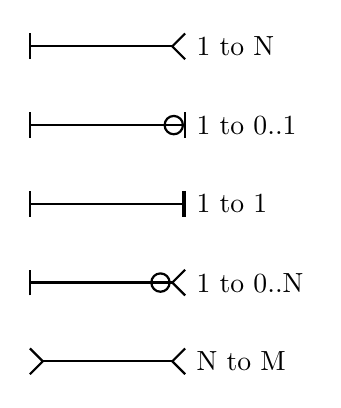
\begin{tikzpicture}
\draw[{|[scale=1.5]}-{Straight Barb[reversed, scale=1.5]}, thick] (0,0) -- (2,0) node[right] {1 to N};
\draw[{|[scale=1.5]}-{Circle[open, scale=1.5] |[scale=1.5]}, thick] (0,-1) -- (2,-1) node[right] {1 to 0..1};
\draw[{|[scale=1.5]}-{|[scale=1.5] |[scale=1.5]}, thick] (0,-2) -- (2,-2) node[right] {1 to 1};
\draw[{|[scale=1.5]}-{Circle[open, scale=1.5] Straight Barb[reversed, scale=1.5]}, thick] (0,-3) -- (2,-3) node[right] {1 to 0..N};
\draw[{Straight Barb[reversed, scale=1.5]}-{Straight Barb[reversed, scale=1.5]}, thick] (0,-4) -- (2,-4) node[right] {N to M};
\end{tikzpicture}
\end{document}
